\documentclass[11pt]{article}
\usepackage{ulem}
\usepackage{fontspec}
\usepackage{multicol}
\usepackage{graphicx}
\DeclareGraphicsExtensions{.pdf,.png,.jpg}
\linespread{1.5}
\setmainfont{Linux Libertine}


\begin{document}
\begin{titlepage}

\newcommand{\HRule}{\rule{\linewidth}{0.5mm}} % Defines a new command for the
\newcommand{\tab}[1]{\hspace{.05\textwidth}\rlap{#1}}
\center % Center everything on the page
 
\textsc{\Large Archbishop Mitty}\\[0.5cm] % Major heading such as course name
\textsc{\large Chemistry Honors}\\[0.5cm] % Minor heading such as course title

%----------------------------------------------------------------------------------------
%	TITLE SECTION
%----------------------------------------------------------------------------------------

\HRule \\[0.4cm]
\textsc{ \huge Iodine Clock Reaction Lab}\\ % Title of your document
\HRule \\[1cm]
 
%----------------------------------------------------------------------------------------
%	AUTHOR SECTION
%----------------------------------------------------------------------------------------

\begin{minipage}{0.4\textwidth}
\begin{flushleft} \large
{\textsc{\emph{Author}}}\\
\textsc{Ritwik Dutta}
\end{flushleft}
\end{minipage}
~
\begin{minipage}{0.4\textwidth}
\begin{flushright} \large
\small{\textsc{\emph{Partners}}}\\
\small{\textsc{Abhijit Ramaprasad}}

\small{\textsc{Aubrey DeHart}} % Supervisor's Name
\end{flushright}
\end{minipage}\\[4cm]

\vfill % Fill the rest of the page with whitespace
\large{\textsc{ \today \space | Hannon 7$^{th}$ | Made with \LaTeX}\\[3cm]}

\end{titlepage}

\section{Purpose}
The purpose of this lab experiment is to:
\begin{itemize}
	\item Help students understand the effects of concentration and temperature on solutions with respect to reactions
\end{itemize}
The chemical reactions that take place in this lab are:
\begin{itemize}
	\item I$_{2}$ (aq) +  H$_{2}$C$_{6}$H$_{6}$O$_{6}$ (aq)  $\rightarrow$ 2H$^{+}$ (aq) + 2 I$^{-}$ (aq) + C$_{6}$H$_{6}$O$_{6}$ (aq)
	\item 2H$^{+}$ (aq) + 2 I$^{-}$ (aq) + H$_{2}$O$_{2}$ (aq) $\rightarrow$ I$_{2}$ (aq) + 2H$_{2}$O (l)
\end{itemize}

\section{Materials and Safety}
\subsection{List of Materials}

\begin{itemize}
	\begin{multicols}{2}
	\item Solution A (pre-prepared)
	\subitem Vitamin C (1 ml) $\times$ 5
	\subitem Tincture of Iodine (2\%,1 ml) $\times$ 5
	\subitem Distilled water (1 ml) $\times$ 60
	\item Glass test tube (50 ml) $\times$ 4
	\item Digital thermometer $\times$1
	\item Solution B (pre-prepared)
	\subitem Hydrogen peroxide (1 ml) $\times$ 15
	\subitem Laundry Starch (1 ml) $\times$ 2
	\subitem Distilled water (1 ml) $\times$ 60
	\item Deionized water squirt bottle $\times$1
	\item Digital stopwatch $\times$1
	\end{multicols}
\end{itemize}
\subsection{Safety Information}
\subsubsection{Vitamin C}
This substance can be dangerous if it comes into contact with skin or eyes. Flush affected eyes with water for at least 15 minutes and seek medical attention. Wash affected skin with soap and water, and cover with an emollient. If irritation develops, seek medical attention\footnote{https://www.sciencelab.com/msds.php?msdsId=9922972}. 
\subsubsection{Tincture of Iodine}
This substance can be dangerous if it comes into contact with the skin or eyes. Flush the affected area with water for at least 15 minutes and get medical attention\footnote{http://www.sciencelab.com/msds.php?msdsId=9924377}. 
\subsubsection{Hydrogen Peroxide}
This substance can be dangerous if it comes into contact with the skin or the eyes. Flush the affected area with water for 15 minutes and get medical attention\footnote{http://www.sciencelab.com/msds.php?msdsId=9924298}. 
\section{Apparatus and Procedure}
\subsection{Apparatus}
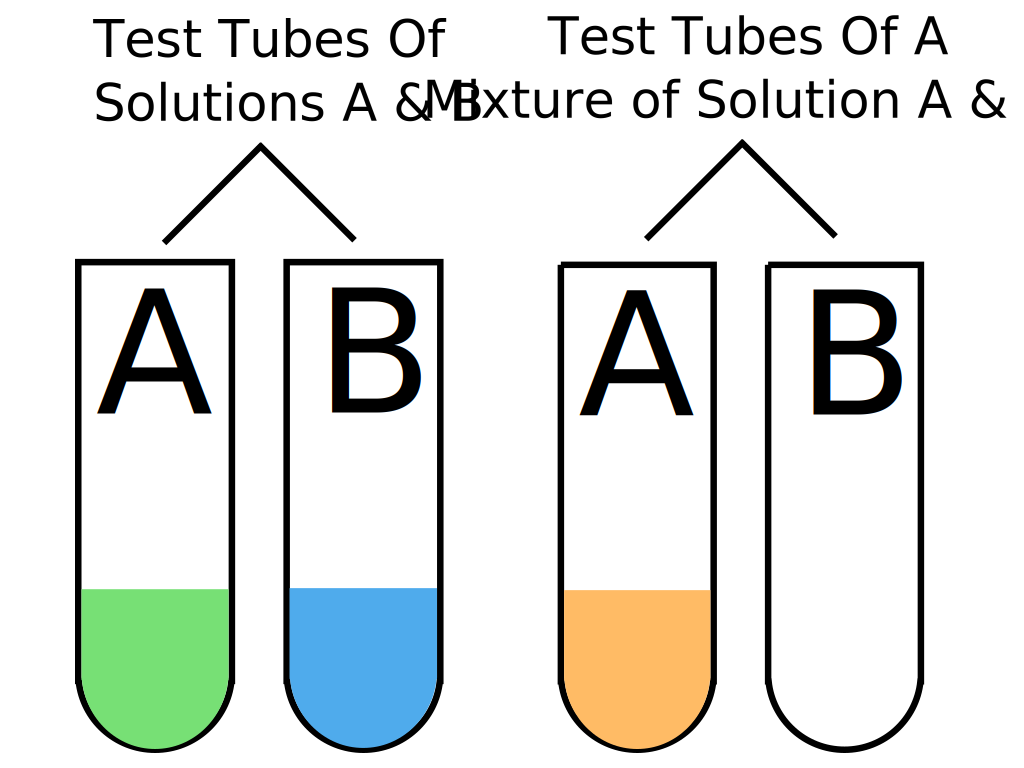
\includegraphics[width=\textwidth]{IodineApp}
\subsection{Procedure}
\subsubsection{The Effect of Concentration Changes }
\begin{enumerate}
\item		Use	a	dial	volumetric	dispenser	attached	to	a	plastic	serological	pipet,	measure	the	given	volume	of	distilled	water,	and	pour	it	into	a	clean,	dry	test	tube	that	
you	have	labeled	“A”. \\ \\
\begin{tabular*}{\textwidth}{ @{\extracolsep{\fill} } l r}
\textbf{\large{Group Number}} & \textbf{\large{Distilled Water}}\\ \hline
	All Groups & 0.0 mL \\ \hline
	1 - 2 	& 5.0 	mL		\\ \hline
	3 - 4 	& 10.0 	mL	\\ \hline
	5 - 6 	& 15.0 	mL\\ \hline
	7 - 8 	& 20.0 	mL	\\ \hline
\end{tabular*} \\
\item With	the	pump	dispenser	at	the	prep	table,	add	5.0	mL	of	Solution	A	to	test	tube	“A”	that	already	contains	the	distilled	water.		Swirl	to	mix.	
	
\item With	the	pump	dispenser	in	the	fume	hood,	measure	5.0	mL	of	Solution	B	into	a	separate	clean,	dry	test	tube	that	you	have	labeled	“B”.			
In	each	case,	the	temperature	(room	temp.)	will	be	kept	constant.	
	
\item Using	a	stopwatch,	press	 the	“start”	button	as	you	pour	solution	A	into	solution	B,	 then	pour	 them	back	and	 forth	quickly	 three	 times	 to	obtain	a	uniform	
mixing.		Time	should	be	recorded	from	the	instant	at	which	both	solutions	are	in	contact.	
	
Observe	the	reaction	carefully,	and	stop	the	timer	\textbf{immediately}	at	the	first	sign	of	a	color	change.	
	
\item Record	 your	reaction	 time	in	 the	appropriate	box	in	 the	data	 table	 for	your	class	(which	 you	will	later	transfer	 to	your	lab	notebook,	along	with	detailed	
observations).		Then,	empty	the	contents	of	each	test	tube	into	the	labeled	hazardous	waste	container.		Rinse	each	test	tube	with	distilled	water,	and	dry	each	
tube	to	the	best	of	your	ability.	
	
\item Each	group	has	been	assigned	two	different	combinations	in	the	above	chart	(the	top	row,	and	one	other).		Repeat	steps	1-4	for	your	second	combination.	
	
\item As	a	class,	record	the	room	temperature	at	which	all	of	these	reactions	have	been	conducted.		This	temperature	will	be	used	for	your	Analysis	section	later.	
\end{enumerate}

\subsubsection{The Effect of Temperature Changes}
\begin{enumerate}
\item Using	the	same	techniques	as	in	Part	1,	dispense	5.0	mL	of	Solution	A	into	your	clean,	dry	“A”	test	tube,	and	dispense	5.0	mL	of	Solution	B	into	your	clean,	dry	
“B”	test	tube.	

\item	These	solutions	must	be	brought	to	the	desired	temperature	before	they	are	mixed.		Put	both	the	“A”	and	“B”	test	tubes	into	a	250-mL	beaker	that	is	about	
two-thirds	full	of	water	at	the	temperature	you	were	assigned	to	investigate.		Let	them	stand	for	about	10	minutes,	so	the	solutions	will	come	to	the	temperature	
of	the	“water	bath”.	\\ \\
\begin{tabular*}{\textwidth}{ @{\extracolsep{\fill} } l r}
\textbf{\large{Group Number}} & \textbf{\large{Approximate Temperature of Solution}}\\ \hline
	All Groups 	& Room Temperature 			\\ \hline
	1 - 2 		& 1$^\circ$		C			\\ \hline
	3 - 4 		& 10$^\circ$ 	C 			\\ \hline
	5 - 6 		& 35$^\circ$ 	C 			\\ \hline
	7 - 8 		& 50$^\circ$ 	C 			\\ \hline
\end{tabular*} \\
\item	Using	a	stopwatch,	press	the	“start”	button	as	you	pour	Solution	A	into	Solution	B,	then	pour	them	back	and	 forth	quickly	three	times	to	obtain	a	uniform	
mixing.		Time	should	be	recorded	from	the	instant	at	which	both	solutions	are	in	contact.	
	
Observe	the	reaction	carefully,	and	stop	the	timer	immediately	at	the	first	sign	of	a	color	change.	
	
\item		Record	 your	reaction	 time	in	 the	appropriate	box	in	 the	data	 table	 for	 your	class	 (which	 you	will	later	 transfer	 to	 your	lab	notebook,	along	with	detailed	
observations).		Then,	empty	the	contents	of	each	test	tube	into	the	labeled	hazardous	waste	container.		Rinse	each	test	tube	with	distilled	water,	and	dry	each	
test	tube	to	the	best	of	your	ability.		Place	both	test	tubes	upside	down	in	your	test	tube	rack,	return	all	materials	to	your	lab	bin,	and	wash	your	hands.
\end{enumerate}

\section{Data Table}
\begin{tabular*}{\textwidth}{ @{\extracolsep{\fill} } l l r r}
\textbf{\large{Substance}} & \textbf{\large{Property}} & \textbf{\large{Value}} & \textbf{\large{Unit}}\\ \hline
	Room 			& Temperature	& 24.4  & $^\circ$C\\ \hline
	Vitamin C		& Amount		& 1.000 & g			\\ \hline
	Stock Solution	& Volume		& 5  	& mL		\\ \hline
	Solution A 		& Volume		& 70 	& mL		\\ \hline

\end{tabular*}

\section{Observations}
	\subsection{Before Reaction}
	Solution A is a translucent yellowish liquid that seems to have a viscosity that is approximately equal to water. Solution B is a transparent and colorless liquid that seems to have a viscosity that is approximately equal to water.
	\subsection{During Reaction}
	When the two solutions react, the mixture in the tube moves toward a dark purple color from a translucent yellowish color. 
	\subsection{After Reaction}
	When Solution A and Solution B are combined, we find that the result is an opaque royal purple liquid with a viscosity approximately equal to water. 		When we disposed of the mixture, the jar which contained it all was an opaque black color. 

\section{Analysis and Results}
\subsection{Analysis and Results}
\subsubsection{Overall Results}
There were two chemical reactions that took place during this experiment:
\begin{itemize}
\item I$_{2}$ (aq) +  H$_{2}$C$_{6}$H$_{6}$O$_{6}$ (aq)  $\rightarrow$ 2H$^{+}$ (aq) + 2 I$^{-}$ (aq) + C$_{6}$H$_{6}$O$_{6}$ (aq)
\item 2H$^{+}$ (aq) + 2 I$^{-}$ (aq) + H$_{2}$O$_{2}$ (aq) $\rightarrow$ I$_{2}$ (aq) + 2H$_{2}$O (l)
\end{itemize}
The molarity of the Vitamin C solution pre-prepared for this experiment is:

	1.000 $\textrm{\sout{g}}$ Vitamin C $\times \frac{\textrm{1 mol}}{\textrm{176.12 \sout{g} } }$ = 0.005678 moles / 0.0700 L = \textbf{0.0811 M}
	
We can determine the molarity of Vitamin C in Solution A to be:

0.0811 M $\times \frac{\textrm{5.0\sout{mL}}}{\textrm{70.0 \sout{mL}}}$ = \textbf{0.0058 M}
	
\subsubsection{Effect of Concentration}
The molarity for each of the trials was:

\begin {itemize}
\item 5.0 mL added water:\\
 0.0058 M $ \times \frac{\textrm{5.0 \sout{mL}}}{\textrm{15.0\sout{mL}}}$ = \textbf{.0019 M}
 \item 10 mL added water:\\
 0.0058 M $ \times \frac{\textrm{5.0 \sout{mL}}}{\textrm{20.0\sout{mL}}}$ = \textbf{.0014 M}
 \item 15 mL added water:\\
 0.0058 M $ \times \frac{\textrm{5.0 \sout{mL}}}{\textrm{25.0\sout{mL}}}$ = \textbf{.0011 M}
 \item 20 mL added water:\\
 0.0058 M $ \times \frac{\textrm{5.0 \sout{mL}}}{\textrm{30.0\sout{mL}}}$ = \textbf{.00097 M}
\end{itemize}
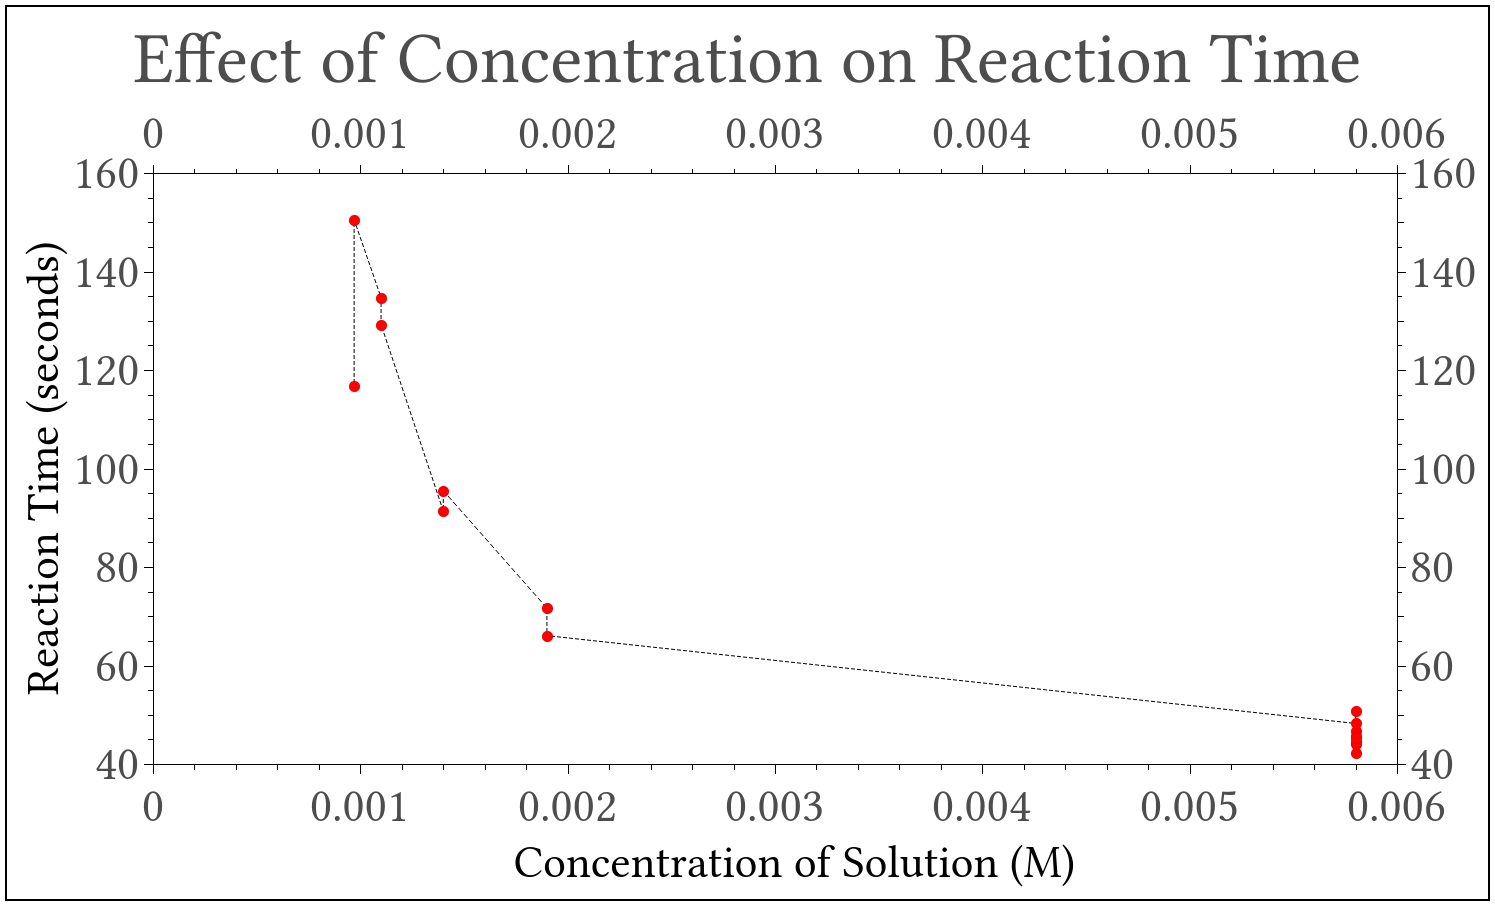
\includegraphics[width=\textwidth]{ConcVsTime}\\
The main thing that this lab teaches me is that as the concentration of a solution decreases, it takes far longer for the reaction to complete. The main reason behind this is that the particles in a certain amount of the solution are decreased, so they are less likely to bump into each other, and thus react. \\
\\
To calculate the average deviation, first we add together all of our reaction times with a concentration of 0.0058 M:
\\
42.21 seconds + 44.08 seconds + 46.6 seconds + 45.61 seconds + 44.44 seconds + 45.26 seconds + 50.68 seconds + 48.23 =\textbf{ 367.11 seconds}\\
\\
Now we divide that value by the total number of times to get:
\\
$ \frac{\textrm{367.11 seconds}}{\textrm{16 total times}}$ = \textbf{45.88875 seconds per time} \\
\\
Next, we take each element, calculate its distance from the average, and add the differences to get:
\\
3.67875 seconds + 1.80875 seconds + 0.71125 seconds + 0.27875 seconds + 1.44875 seconds + 0.62875 seconds + 4.79125 seconds + 2.34125 seconds = \textbf{15.6875 seconds}\\
\\
Now we divide that value by the total number of times to get:
\\
$ \frac{\textrm{15.6875 seconds of deviation}}{\textrm{16 total times}}$ = \textbf{1.961 seconds of average deviation} \\
\\
This average deviation is a relatively small value. It is equal to about 4.273\% of the average reaction time, and therefore I believe that the method used to determine the reaction time was precise. However, there is an inherent imprecision in the fact that the starting and stopping points of time measurement were controlled by human reaction time, which is fundamentally limited. If this footage was instead videotaped and then timed by using reference points in the resulting video file, I believe that the precision of time measurement would be higher.  


\subsubsection{Effect of Temperature}

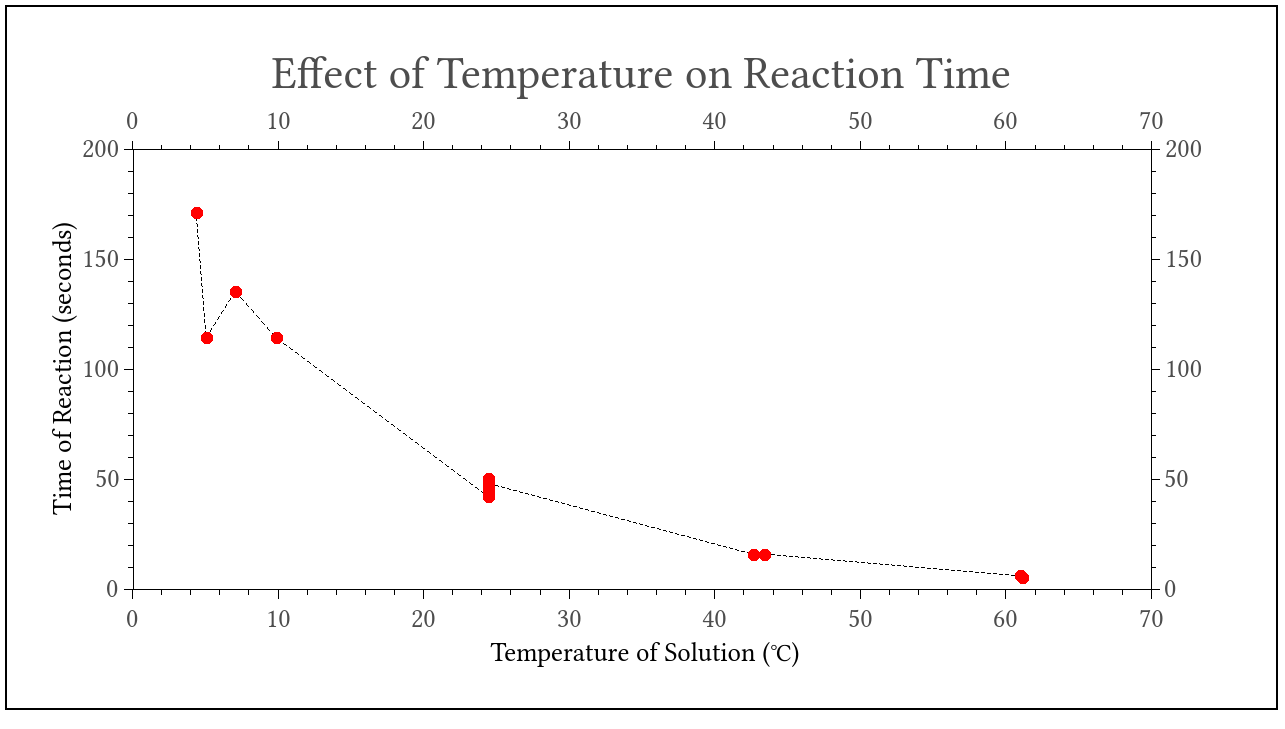
\includegraphics[width=\textwidth]{TempvsTime}\\
The main thing that this lab has taught me is the fact that as the temperature of a solution increases, the speed at which a reaction occurs is increased. As the temperature of the particles in the solution goes up, the average amount of energy, and thus the speed at which they move, goes also rises, and thus they are far more likely to bump into one another and thus react.\\
\\
Another possible way to increase the speed of reaction would be to use elements which are more reactive because then the reaction occur far quicker because the particles in those elements would be moving far faster at the same temperature more, and thus increase the speed at which the reaction occurs.

\subsection{Results Table}
\begin{tabular*}{\textwidth}{ @{\extracolsep{\fill} }  l  r }
\textbf{\large{Total Volume of Solution (mL)}} & \textbf{\large{Molarity of Vitamin C (M)}} \\ \hline
10.0 mL & .0058  \\ \hline
15.0 mL & .0019  \\ \hline
20.0 mL	& .0014  \\ \hline
25.0 mL	& .0011  \\ \hline
30.0 mL	& .00097 \\ \hline
\end{tabular*}
\\
\\
\\
\begin{tabular*}{\textwidth}{ @{\extracolsep{\fill} }  l r r }
\textbf{\large{Property}} & \textbf{\large{Value}} & \textbf{\large{Units}} \\ \hline
Average Deviation 								& 1.961  	& seconds \\ \hline
Average Reaction Time (10mL, Room temperature) 	& 45.89  	& seconds \\ \hline
\end{tabular*}
\\
\section{Conclusions}

\subsection{Conclusions}
This lab teaches students about the catalysts that can affect the speed of a reaction, as well as about the concentration and dilution calculations necessary to determine the molarities of solutions. Although there is no percent error because there was no definitive time known for the used elements, several sources of error can nevertheless be obtained and analyzed. One of the more likely sources of error stems from the fact that these tubes used to perform the experiment were not pure - they had been cleaned with water, and thus there might have been more water in the solution than there should have been. This would have increased the concentration, and thus icnreased the time of reaction, thus classifying it as a positive error. Another likely source of error stems from the fact that Some of either Solution A or Solution B could have been spilled in the process of being poured back and forth between the two test tubes. If some liquid fell out, the concentration would again decrease, thus increasing the time, and thus also classfying this source of error as a positive error. 

\end{document}
